\chapter{Finding Optimal Hyperparameters for the Cleaning Algorithms}
\label{ch:finding-hyperparams}

This work aims to find optimal hyperparameters for the cleaning algorithms used in \ctapipe{}.
Optimizing the cleaning step (see \autoref{sec:data-levels}) can most certainly lead to a better
reconstruction of the events in a dataset. Therefore a tweaking of the available parameters of each
cleaner is necessary. In this chapter, I will first introduce the cleaning algorithms and their parameters
in \autoref{sec:cleaning-algorithms} and then describe the procedure to find optimal hyperparameters
in \autoref{sec:hyperparameters}.

\section{Cleaning Algorithms}
\label{sec:cleaning-algorithms}

Version \texttt{0.15.1} of \ctapipe{} features four cleaning algorithms, two of which are time-based.
The \tailcuts{} algorithm is the most basic algorithm of the four and serves as a good
starting point for the development of new cleaning algorithms. Its first step is to select all
pixels that are above a certain threshold, the \texttt{picture} or \texttt{core\_threshold}. These
pixels are the core part of the signal and are the brightest. The \tailcuts{} algorithm
then selects all pixels that are above the so-called \texttt{boundary\_threshold} and are neighboring
the core pixels. A visualization of the algorithm is shown in \autoref{fig:tailcuts_clean} for the
default values of the algorithm.

\begin{figure}
    \centering
    \begin{subfigure}[t]{0.33\textwidth}
        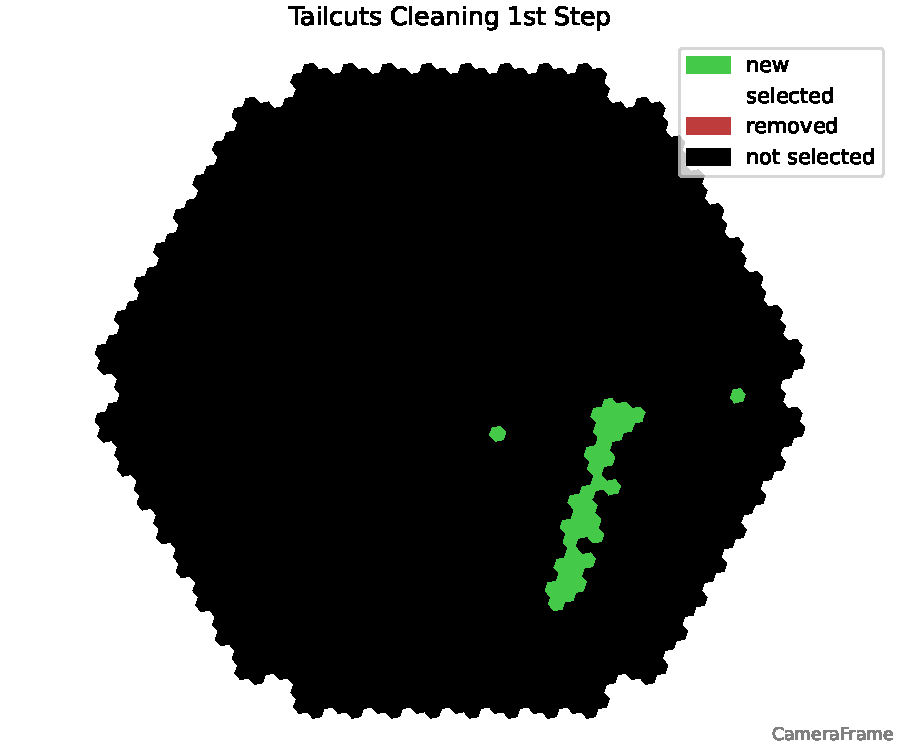
\includegraphics[width=\textwidth]{plots/cleaner_steps/tail_1.pdf}
    \end{subfigure}
    \begin{subfigure}[t]{0.33\textwidth}
        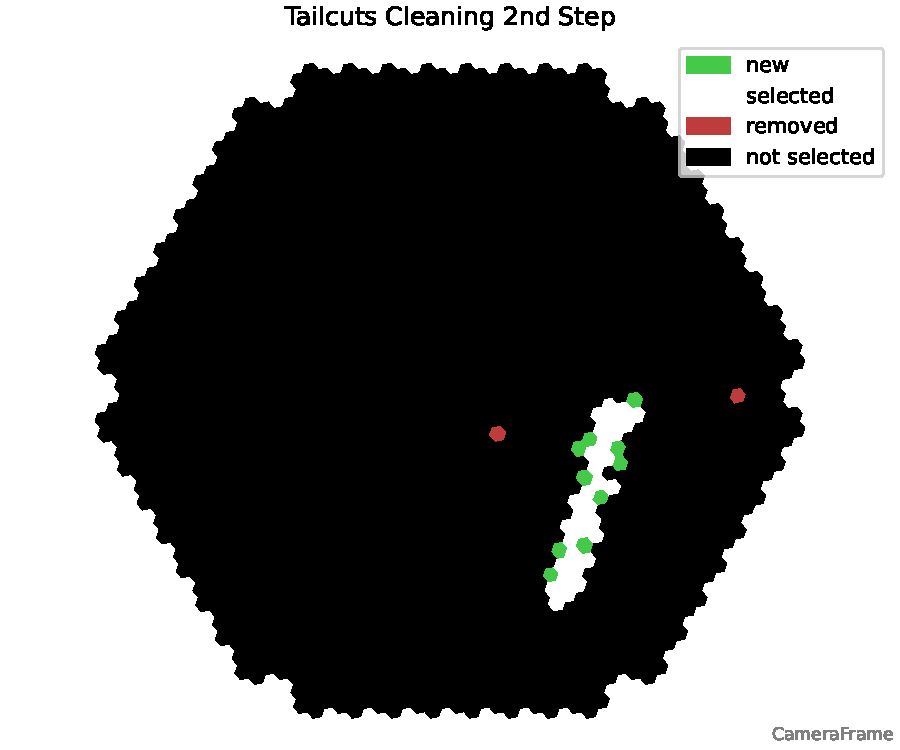
\includegraphics[width=\textwidth]{plots/cleaner_steps/tail_2.pdf}
    \end{subfigure}
    \caption{Visualization of the \tailcuts{} algorithm for a \gls{mst} NectarCam image. First, all
    pixels above the \texttt{core\_threshold} are selected. Then, all pixels neighboring the core
    pixels that are above the \texttt{boundary\_threshold} are selected.}
    \label{fig:tailcuts_clean}
\end{figure}

The \mars{} algorithm is very much based on the \tailcuts{}
algorithm and features an additional step, in that it also selects all neighbors of a neighbor of a
core pixel, if they are above the \texttt{boundary\_threshold}. The three steps for the \mars{} algorithm
are shown in \autoref{fig:mars_cleaning} for the default values of the algorithm.

\begin{figure}
    \centering
    \begin{subfigure}[t]{0.32\textwidth}
        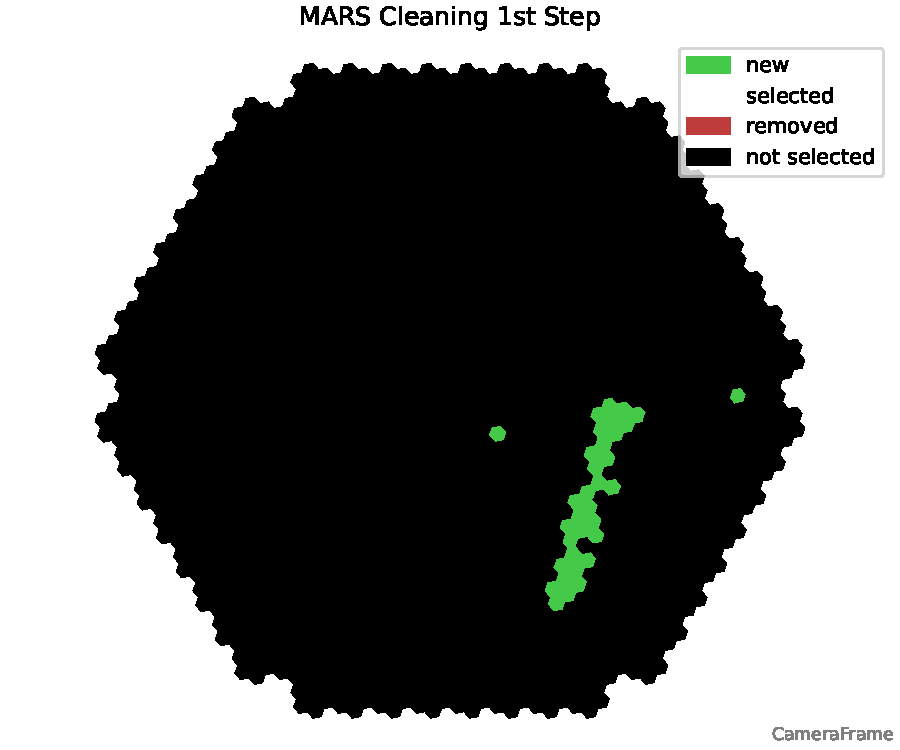
\includegraphics[width=\textwidth]{plots/cleaner_steps/mars_1.pdf}
    \end{subfigure}
    \hfill
    \begin{subfigure}[t]{0.32\textwidth}
        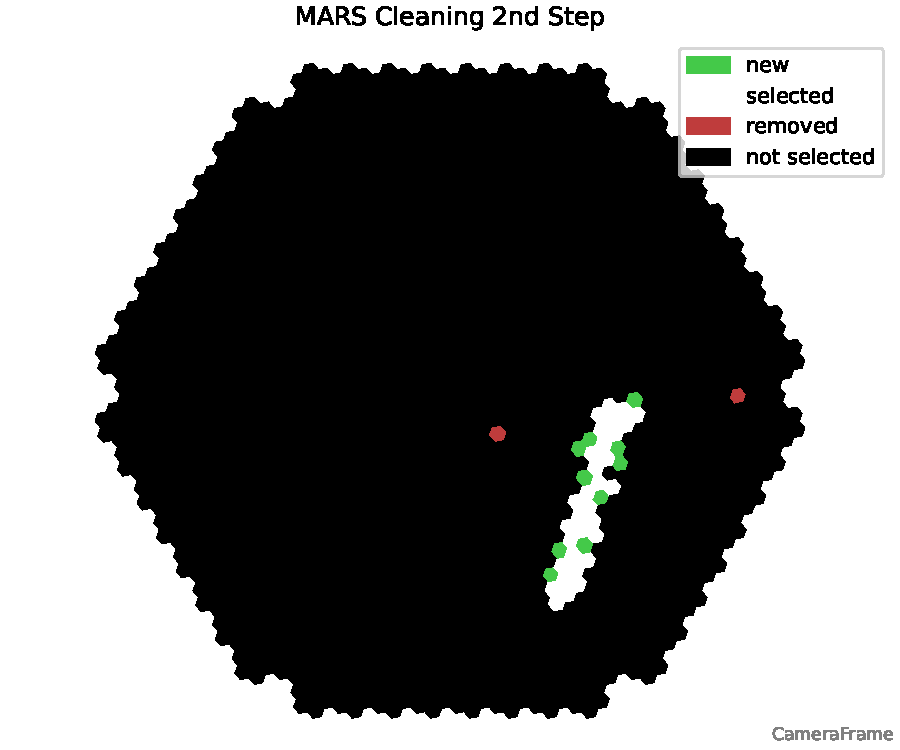
\includegraphics[width=\textwidth]{plots/cleaner_steps/mars_2.pdf}
    \end{subfigure}
    \hfill
    \begin{subfigure}[t]{0.32\textwidth}
        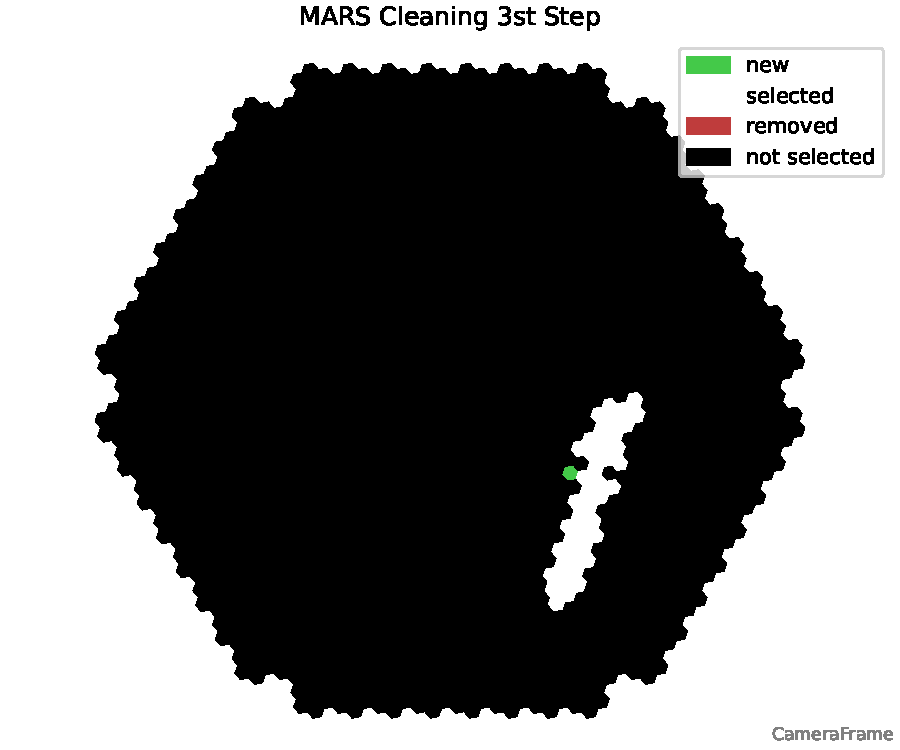
\includegraphics[width=\textwidth]{plots/cleaner_steps/mars_3.pdf}
    \end{subfigure}
    \caption{Visualization of the \mars{} algorithm for a \gls{mst} NectarCam image. The first two
    steps are identical to the \tailcuts{} algorithm. The third step selects all neighbors of a neighbor of a
    core pixel, if they are above the \texttt{boundary\_threshold}.}
    \label{fig:mars_cleaning}
\end{figure}

The \fact{} algorithm is a time-based cleaning algorithm that first selects all pixels that are above
the \texttt{core\_threshold}. Then, all pixels that have less than \(N\) neighbors are removed. The
\texttt{min\_number\_neighbors} parameter is set to \(\num{2}\) by default. For the third step, all pixels neighboring
the remaining pixels that are above the \texttt{boundary\_threshold} are selected. After that, all
pixels that have less than \(N\) neighbors and that have arrived within a given timeframe are removed.
The \texttt{time\_limit} parameter is set to \(\SI{5}{\nano\second}\) by default. Again, all pixels
with less than \(N\) neighbors are removed. The last step once again removes pixels with less than
\(N\) neighbors, arriving within the given time limit. The visualization of the algorithm is shown in
\autoref{fig:fact_cleaning} for the default values of the algorithm.

\begin{figure}
    \centering
    \begin{subfigure}[t]{0.32\textwidth}
        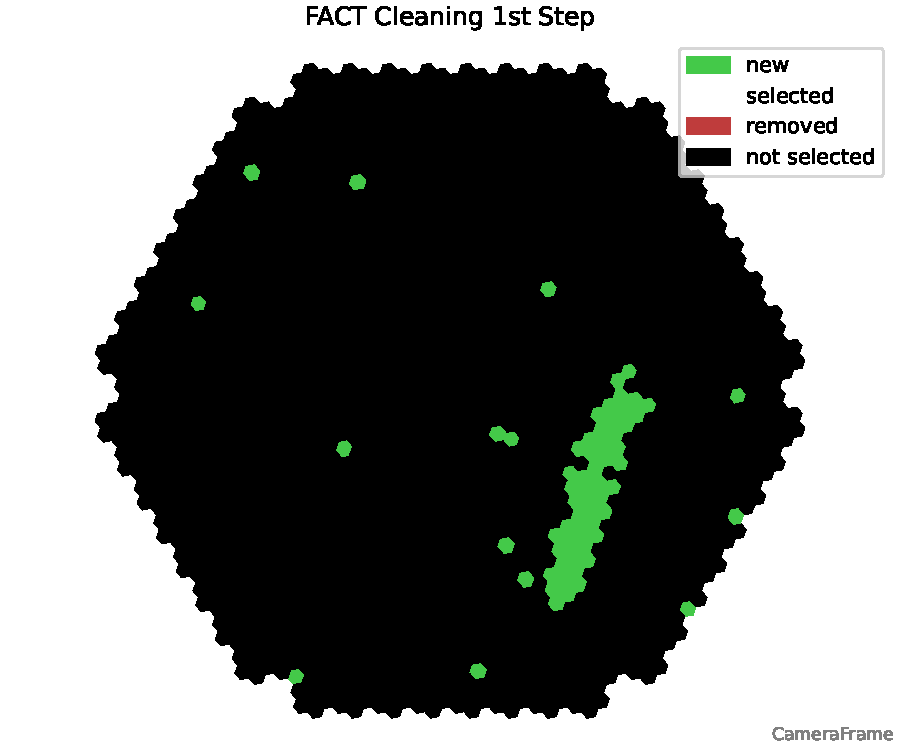
\includegraphics[width=\textwidth]{plots/cleaner_steps/fact_1.pdf}
    \end{subfigure}
    \hfill
    \begin{subfigure}[t]{0.32\textwidth}
        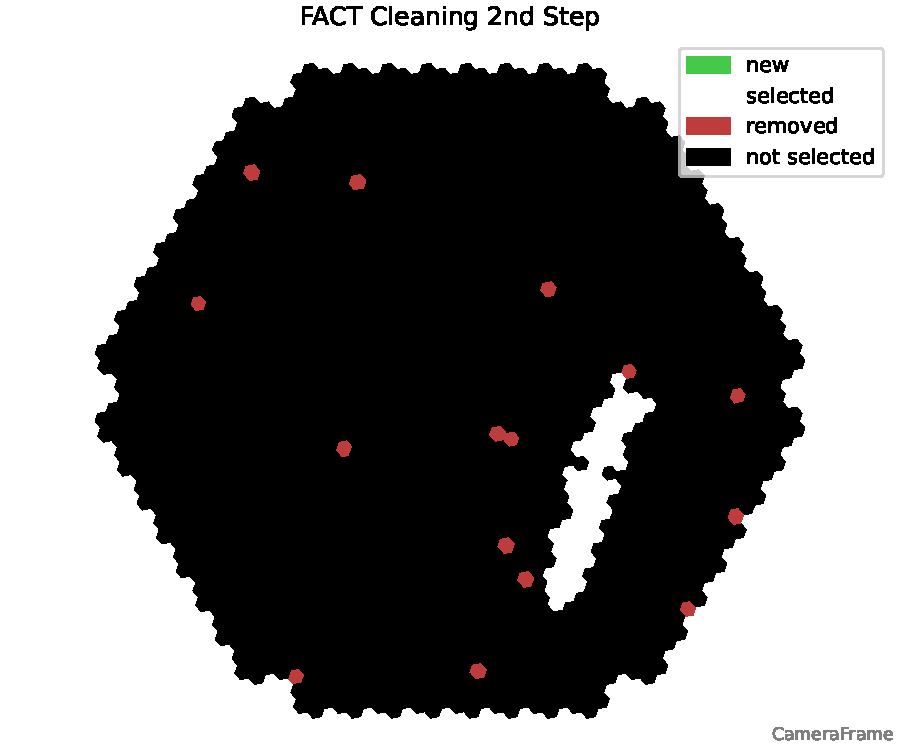
\includegraphics[width=\textwidth]{plots/cleaner_steps/fact_2.pdf}
    \end{subfigure}
    \hfill
    \begin{subfigure}[t]{0.32\textwidth}
        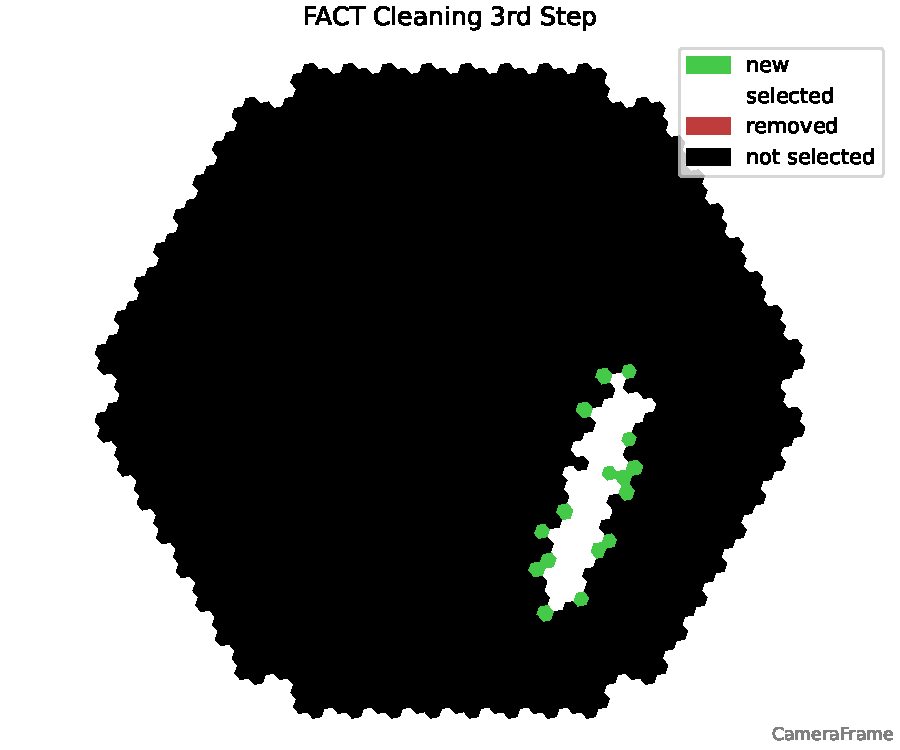
\includegraphics[width=\textwidth]{plots/cleaner_steps/fact_3.pdf}
    \end{subfigure}
    \begin{subfigure}[b]{0.32\textwidth}
        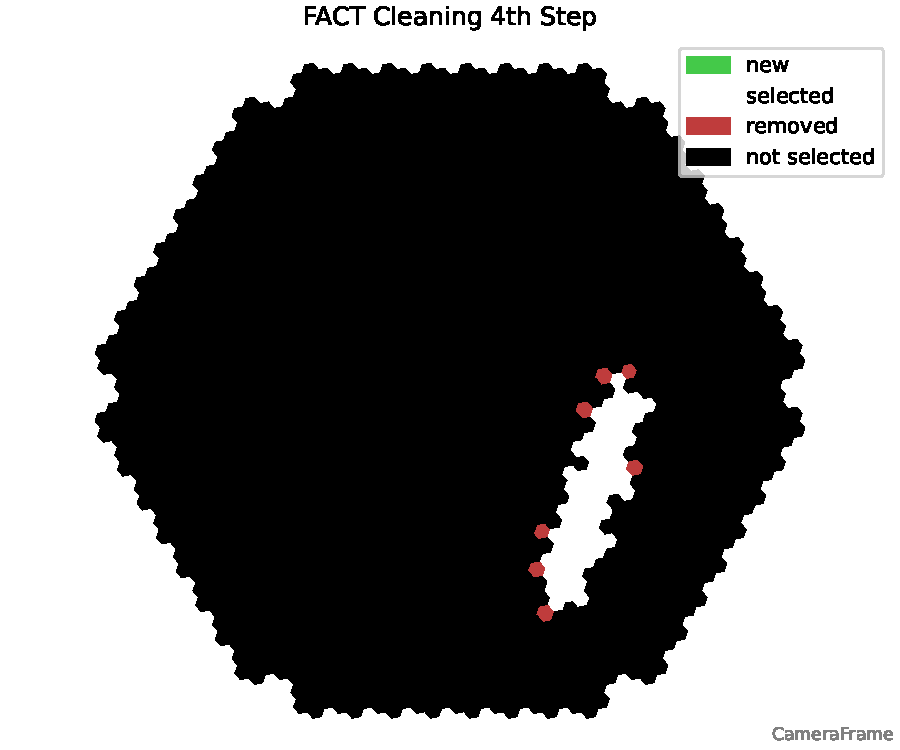
\includegraphics[width=\textwidth]{plots/cleaner_steps/fact_4.pdf}
    \end{subfigure}
    \hfill
    \begin{subfigure}[b]{0.32\textwidth}
        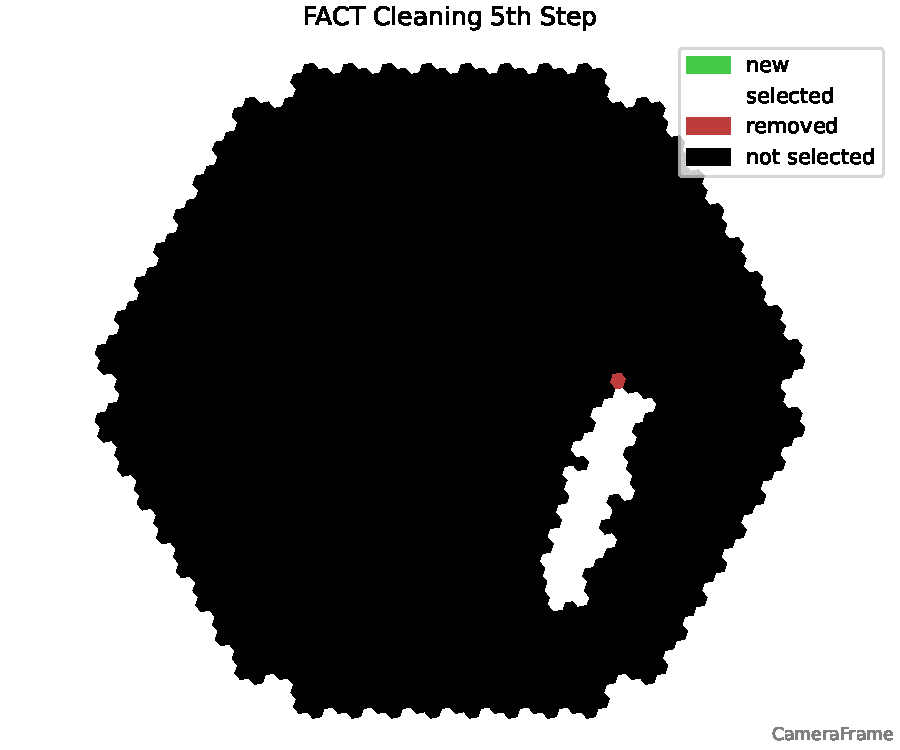
\includegraphics[width=\textwidth]{plots/cleaner_steps/fact_5.pdf}
    \end{subfigure}
    \hfill
    \begin{subfigure}[b]{0.32\textwidth}
        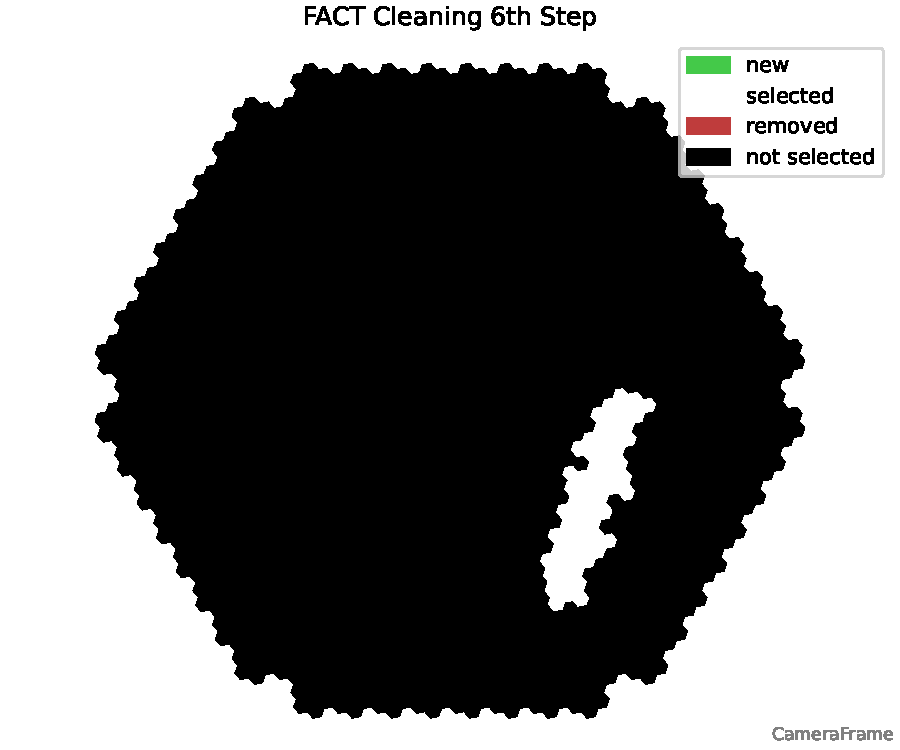
\includegraphics[width=\textwidth]{plots/cleaner_steps/fact_6.pdf}
    \end{subfigure}
    \caption{Visualization of the \fact{} algorithm for a \gls{mst} NectarCam image. The first
    step selects all pixels above the \texttt{core\_threshold}. The second step removes all pixels that have less than
    \(N\) neighbors. The third step selects all pixels neighboring the remaining pixels that are above the
    \texttt{boundary\_threshold}. The fourth step removes all pixels that have less than \(N\) neighbors,
    that have arrived within a given timeframe. The fifth and sixth steps are analogous to steps two and four.}
    \label{fig:fact_cleaning}
\end{figure}

The \tcc{} algorithm is another time-based algorithm, coming from the \gls{magic} collaboration.
It first selects all pixels that are above the \texttt{core\_threshold}. Then, all pixels that have
less than \(N\) neighbors are removed. The \texttt{min\_number\_neighbors} parameter is set to \(\num{1}\) by default.
After that, all core pixels whose arrival times are within a given timeframe of the average arrival time.
This \texttt{time\_limit\_core} parameter is set to \(\SI{4.5}{\nano\second}\) by default. As a fourth step,
the \tcc{} algorithm finds all pixels above the \texttt{boundary\_threshold}. Then, all pixels with
less than \(N\) neighbors arriving within a given timeframe are removed. This \texttt{time\_limit\_boundary}
parameter is set to \(\SI{1.5}{\nano\second}\) by default. The visualization of the algorithm is shown in
\autoref{fig:tcc_cleaning} for the default values of the algorithm.

\begin{figure}
    \centering
    \begin{subfigure}[t]{0.32\textwidth}
        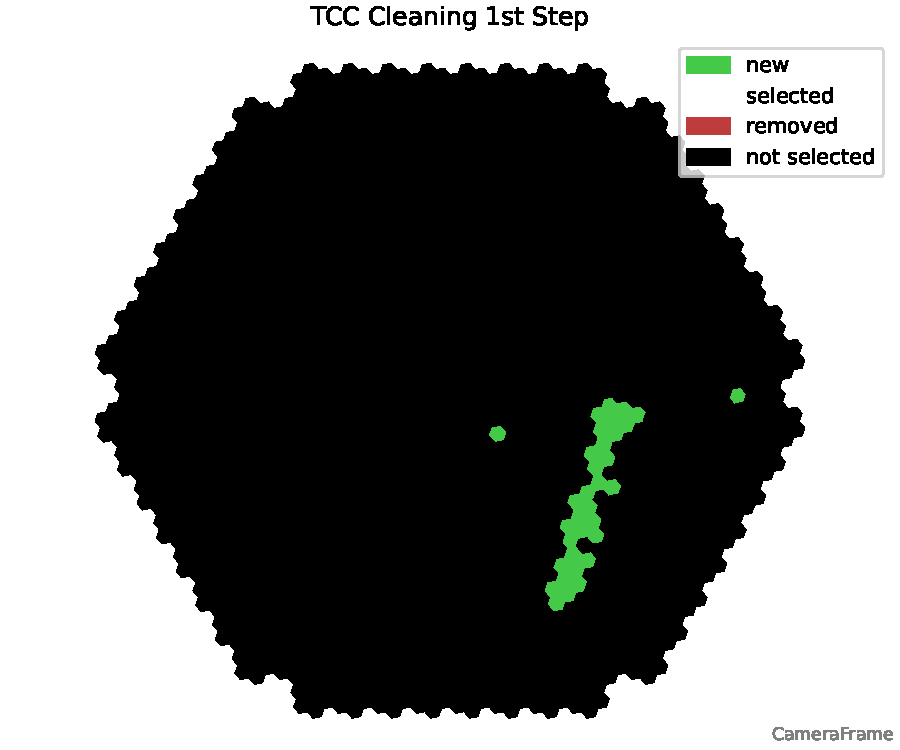
\includegraphics[width=\textwidth]{plots/cleaner_steps/tcc_1.pdf}
    \end{subfigure}
    \hfill
    \begin{subfigure}[t]{0.32\textwidth}
        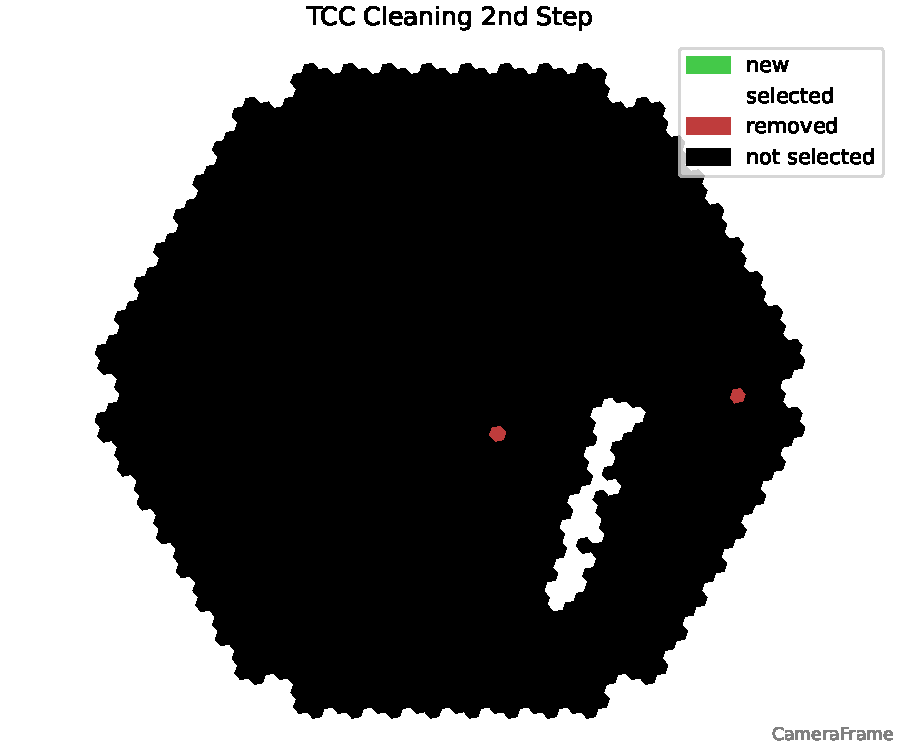
\includegraphics[width=\textwidth]{plots/cleaner_steps/tcc_2.pdf}
    \end{subfigure}
    \hfill
    \begin{subfigure}[t]{0.32\textwidth}
        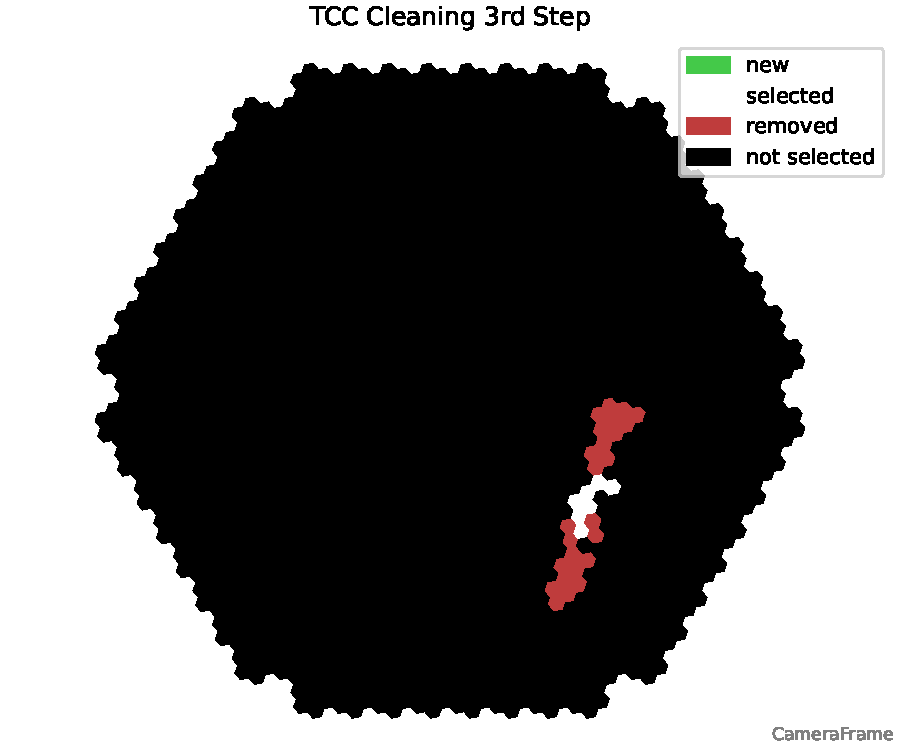
\includegraphics[width=\textwidth]{plots/cleaner_steps/tcc_3.pdf}
    \end{subfigure}
    \begin{subfigure}[]{0.32\textwidth}
        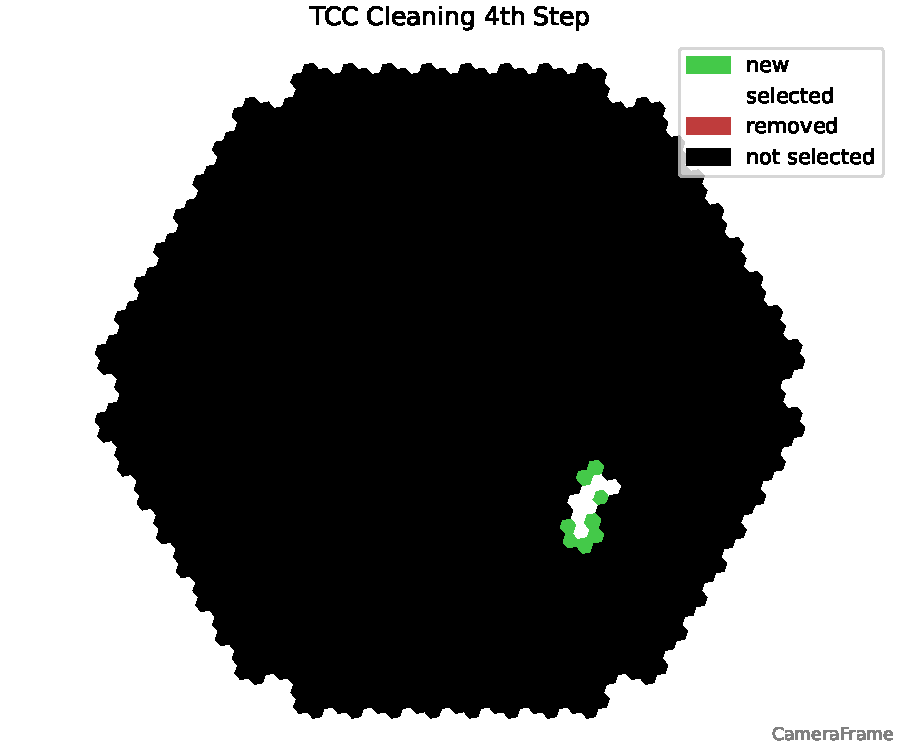
\includegraphics[width=\textwidth]{plots/cleaner_steps/tcc_4.pdf}
    \end{subfigure}
    \begin{subfigure}[]{0.32\textwidth}
        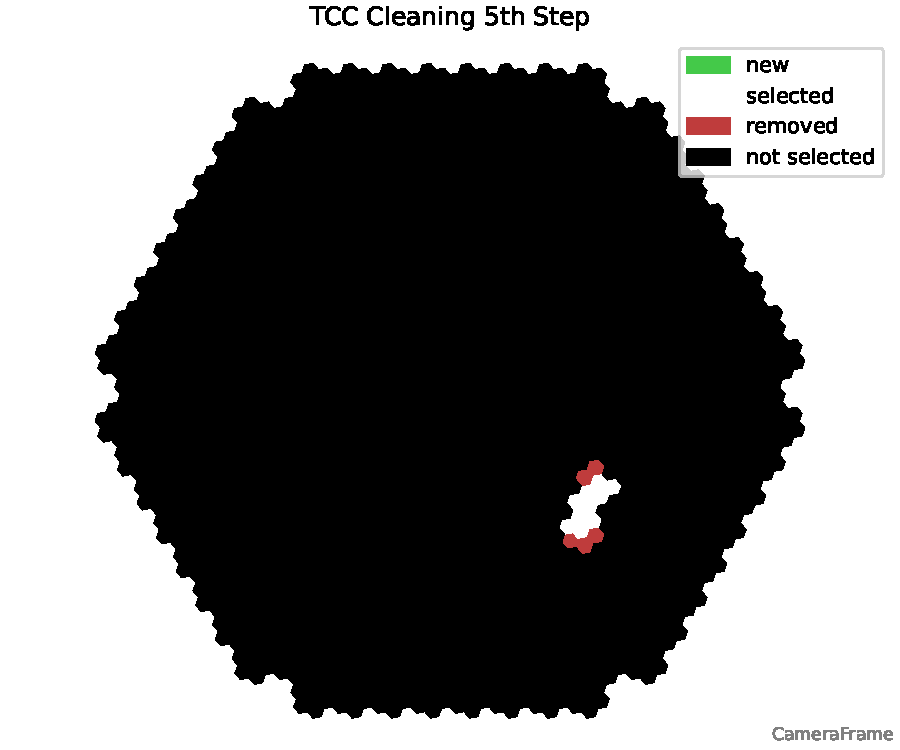
\includegraphics[width=\textwidth]{plots/cleaner_steps/tcc_5.pdf}
    \end{subfigure}
    \caption{Visualization of the \tcc{} algorithm for a \gls{mst} NectarCam image. The first step
    selects all pixels above the \texttt{core\_threshold}. The second step removes all pixels that have less than
    \(N\) neighbors. The third step selects all pixels whose arrival times are within a given timeframe of the
    \texttt{time\_limit\_core} parameter. The fourth step selects all pixels above the \texttt{boundary\_threshold}.
    The fifth step removes all pixels with less than \(N\) neighbors, that have arrived within a given timeframe
    of the \texttt{time\_limit\_boundary} parameter.}
    \label{fig:tcc_cleaning}
\end{figure}

\section{Hyperparameters}
\label{sec:hyperparameters}

The hyperparameters of each cleaning algorithm are set in a specific \texttt{config} file. There,
the user can set and change the parameters, shown in \autoref{tab:hyperparameters}. \tailcuts{}
and \mars{} can be set-up with only three parameters: the \texttt{picture\_threshold}, the
\texttt{boundary\_threshold} and \texttt{min\_number\_picture\_neighbors}. The time-based algorithms
have additional parameters: a \texttt{time\_limit} for \fact{} and a \texttt{time\_limit\_core} as
well as a \texttt{time\_limit\_boundary} for \todo{watch out for text boundaries}\tcc{}.
\begin{table}
    \centering
    \caption{The four cleaning algorithms and their hyperparameters. Being the most basic algorithms,
    \tailcuts{} and \mars{} have only three parameters, while the \fact{} and \tcc{} algorithms have
    one and two additional time-based parameters, respectively. This table shows the default values,
    as they are implemented in the \ctapipe{} source code for version \texttt{0.15.1}.}
    \label{tab:hyperparameters}
    \rowcolors{0}{white!92!black}{}
    \begin{tabular}{l l l}
        \hiderowcolors
        \textbf{Cleaning Algorithm} & \textbf{Hyperparameter} & \textbf{Default Values} \\
        \showrowcolors
        \tailcuts{} & \texttt{picture\_threshold}               & \qquad\(\SI{7}{\pe}\) \\
                    & \texttt{boundary\_threshold}              & \qquad\(\SI{5}{\pe}\) \\
                    & \texttt{min\_number\_picture\_neighbors}  & \qquad\(\num{0}\) \\
        \addlinespace[0.5em]
        \mars{}     & \texttt{picture\_threshold}               & \qquad\(\SI{7}{\pe}\) \\
                    & \texttt{boundary\_threshold}              & \qquad\(\SI{5}{\pe}\) \\
                    & \texttt{min\_number\_picture\_neighbors}  & \qquad\(\num{0}\) \\
        \addlinespace[0.5em]
        \fact{}     & \texttt{picture\_threshold}               & \qquad\(\SI{4}{\pe}\) \\
                    & \texttt{boundary\_threshold}              & \qquad\(\SI{2}{\pe}\) \\
                    & \texttt{time\_limit}                      & \qquad\(\SI{5}{\nano\second}\) \\
                    & \texttt{min\_number\_picture\_neighbors}  & \qquad\(\num{2}\) \\
        \addlinespace[0.5em]
        \tcc{}      & \texttt{picture\_threshold}               & \qquad\(\SI{7}{\pe}\) \\
                    & \texttt{boundary\_threshold}              & \qquad\(\SI{5}{\pe}\) \\
                    & \texttt{time\_limit\_core}                & \qquad\(\SI{4.5}{\nano\second}\) \\
                    & \texttt{time\_limit\_boundary}            & \qquad\(\SI{1.5}{\nano\second}\) \\
                    & \texttt{min\_number\_picture\_neighbors}  & \qquad\(\num{1}\) \\
  \end{tabular}
\end{table}

To find the optimal hyperparameters I used the \texttt{ParameterGrid} class from the
\texttt{sklearn.model\_selection} module \cite{scikit-learn}. The \texttt{ParameterGrid} class is useful to create a
dictionary of all possible combinations of a list of given parameters. These combinations are then
written to a config file and processed with \ctapipe{}. The output is hundreds of datasets equal to
the number of combinations of the given parameters, each with a different setting for the cleaning
performed on the data. The listing below shows the parameters fed into the \texttt{ParameterGrid}:

\begin{minipage}{\textwidth}
    \begin{mdframed}[backgroundcolor=white!20!black,leftmargin=0cm,rightmargin=0cm, skipabove=0pt, innerleftmargin=0,innerrightmargin=0,]
    \begin{pythonlst}
        common_params = {
            "picture_quantiles": (0.995, 0.999, 0.9992, 0.9995, 0.9997, 0.9999),
            "boundary_threshold_ratio": (1/4, 1/3, 1/2, 2/3, 3/4),
            "min_number_picture_neighbors": (1, 2, 3, 4, 5)
        }

        fact_params = {
            "time_limit": (1.0, 2.0, 4.0, 5.0, 6.0, 10.0, 12.0)
        }

        tcc_params = {
            "time_limit_core": (9.0, 12.0, 15.0, 18.0, 20.0),
            "time_limit_boundary" = (4.5, 9.0, 12.0, 15.0)
        }
    \end{pythonlst}
    \end{mdframed}
  \end{minipage}

The name \texttt{common\_params} is used here to refer to the dictionary of parameters that are common
to all cleaning algorithms, while \texttt{fact\_params} and \texttt{tcc\_params} denote the additional
hyperparameters exclusive to \fact{} and \tcc{}. This results in \(\num{150}\) combinations for
\tailcuts{} and \mars{}, \(\num{1050}\) combinations for \fact{} and \(\num{3000}\) combinations for \tcc{}.

Since it's impossible to find the optimal settings just by looking at the
cleaned images of the datasets, a combined metric is necessary to evaluate each cleaner's performance
for the parameter combinations.

In this work, I chose to first look at the efficiency
\begin{equation}
    \eff =  \frac{n_{\mathrm{reco}}}{n_{\mathrm{total}}},
\end{equation}
where \(n_{\mathrm{reco}}\) is the number of reconstructed events and \(n_{\mathrm{total}}\)
the total number of events in the dataset. By taking the mean of the efficiency, one can sort the
datasets by setting upper and lower bounds for the efficiency. The intervals lengths were chosen as
\(\num{0.05}\), \ie \(\SI{5}{\percent}\), resulting in a total of \(\num{20}\) intervals.

For each interval, the mean angular resolution is calculated. The dataset with the lowest mean angular
resolution is the best performing for each interval. Not all events will ever be properly reconstructed
for any parameter combination, so there won't be a mean angular resolution for all intervals, but only
a subset. Also, the mean angular resolution may be higher when more events were reconstructed.
As a result, a trade-off between efficiency and angular resolution is necessary.

